\documentclass[10pt,letterpaper]{article}
%\usepackage[margin=1in,footskip=0.25in]{geometry}
\usepackage{geometry}
\usepackage{mathpazo}
\geometry{top=0.5in, left=0.5in, right=0.5in, bottom=1in}
\usepackage[parfill]{parskip}    		% Begin paragraphs with an empty line rather than an indent
\usepackage{algorithm}
\usepackage{algpseudocode}
\usepackage{multicol}
\setlength\columnsep{20pt}
\usepackage{graphicx}
\usepackage[font={sf,normalsize},labelfont={sf,bf},justification=centering,singlelinecheck=false]{caption}
\usepackage[scaled]{helvet}
\usepackage[colorlinks=true,linkcolor=blue]{hyperref}

\newenvironment{Figure}
{\par\medskip\noindent\minipage{\linewidth}}
{\endminipage\par\medskip}


\begin{document}

\captionsetup[figure]{labelformat=simple, labelsep=quad, labelfont={sf, bf}}
\captionsetup[table]{ labelformat=simple, labelsep=quad, labelfont={sf, bf}}

\begin{center}
\textbf{\LARGE Multi-Fare Airline Ticket Dynamic Pricing Using Model-Free Reinforcement Learning}

{\Small Group 117 - Final Project Status Update \\ \Small Ross B. Alexander, Jonathan S. Ling}
\end{center}

\begin{multicols*}{2}

\section*{Background}
Dynamic pricing in the airline industry demonstrates some of the most effective pricing schemes in business to maximize revenue based on customers' willingness to pay for particular goods at particular times. We propose to develop a dynamic pricing reinforcement learning algorithm to maximize revenue for a single flight with multiple customer segments. We suggest reinforcement learning as it is a model-free paradigm and thus less sensitive to unusual demand patterns, and because it is a relatively new approach to dynamic pricing for airlines.

This is a decision-making problem under uncertainty that has two distinct perspectives - airline and customer. The airline must determine what prices to set without knowing the underlying stochastic demand functions of customers. In seeking to maximize revenue, the airline must balance the need to sell all their seats before the departure date with waiting until the last minute to sell their most expensive seats. The customer, in seeking to obtain a single ticket at the lowest cost, has the opportunity to learn from the advertised prices over time in order to estimate the best time to purchase a ticket, but must also purchase a ticket before all tickets are gone.

%Need to describe problem again here. How we formulated an approach to solving the problem. Timeline to completion, etc. 

\section*{Problem Formulation}
We formulate a Markov decision process (MDP) with the following 'sub-MDPs' for each fare class $f \in F = \{ 1,2,3 \}$ as follows:

\begin{itemize}
    \item States $(v, u, h) \in \mathcal{S}_f$ are composed of the total number of tickets vacant (available) $v \in [0,V]$, the number of tickets utilized (sold) in the $f$ fare class $u \in [0,U_f]$, and the remaining horizon to sell tickets $h \in [0,H]$
    \item Actions $a \in \mathcal{A}_f$ are ticket price assignments for the corresponding fare class, where each fare class price list $\mathcal{A}_f$ contains 30 prices in increments of \$10 with the upper and lower price bounds set by the fare class
    \item Reward $r \in \mathcal{R}$ is the revenue, or sum over all fare classes of the product of the fare class' ticket price and quantity of tickets sold at each time step
\end{itemize}

We then solve an overarching MDP that summarizes all fare classes together. It differs from the fare class-specific MDPs in the following ways:

\begin{itemize}
    \item States $(v, h) \in \mathcal{S}$ have no $u$ variable
    \item Actions $(a_1,a_2,...,a_|F|) \in \mathcal{A}$ are now vectors of size $|F|$ to denote the prices set by fare class
\end{itemize}

Also, in place of a dataset, we formulate a generative model $(s',r) \sim G_f(s,a)$, to simulate the demand and purchase of tickets in each fare class $f$.

In addition, we define the following quantities:
\begin{itemize}
    \item $n$ is the number of new customers at the current time step
    \item $C$ is the (initially empty) set of all customers seeking tickets at the current time step (i.e., new customers from past time steps that did not purchase, plus all new customers from the current time step)
    \item $w_i$ is customer $i$'s $50 \%$ willingness-to-pay (WTP) threshold
    \item $k_i$ is customer $i$'s WTP flexibility
    \item $\phi_i$ is the likelihood that customer $i$ buys at price $a$
    \item $b_i \in \{ 0,1 \}$ indicates whether customer $i$ in fare class $f$ bought the ticket (1) or not (0)
\end{itemize}

We use \hyperref[alg:generative-model]{Algorithm 1} as our generative model. At each time step, we select some number of new customers from a Poisson distribution (with a linearly decreasing mean), randomly generate their WTP characteristics, and from this, determine how many tickets get sold.

\begin{algorithm}[H]
\label{alg:generative-model}
	\caption{\textsc{GenerativeModel$_f (s (v, u, h), a)$}}
	\small\begin{algorithmic}[1]
	    \State $u' \leftarrow 0$
	    \State $n \sim \textnormal{Poisson}(\alpha_f (H-h) + \beta_f)$ for some constants $\alpha_f, \beta_f$ % number of new customers
        \For {$i$ in $1$ to $n$} % do for all new customers
            \State $w_{i} \sim \mathcal{N}({\mu_w}_f, {\sigma_w}_f)$
            \State $k_{i} \sim \mathcal{N}({\mu_k}_f, {\sigma_k}_f)$
            \State $C \leftarrow C \cup \{i\}$
        \EndFor
        \For {$i \in C$} % do for all customers including new and old customers without tickets
            \State $\phi_{i} = 1 - \textnormal{CDF(Logistic}(a \mid w_i, k_i))$
            \State $b_i \sim \textnormal{Bernoulli}(1,\phi_i)$
            \If{$b_i$ = 1} % sell a ticket and remove the customer
                \State $u' \leftarrow u' + 1$
                \State $C \leftarrow C \setminus \{i\}$
            \EndIf
        \EndFor
	    \State ${r} \leftarrow a \cdot u'$       
		\State\Return {($(v-u',u',h-1),r$)}
	\end{algorithmic}
\end{algorithm}

We have chosen distributions over each of the random variables in a way that represents the problem dynamics. In some cases, such as the customer's WTP threshold and WTP flexibility, alternative distributions can also be justified. The customer's WTP is modeled as a complementary cumulative distribution function for the logistic distribution. The following figures depict the customer pricing dynamics and customer arrival dynamics.

\begin{Figure}
    \centering
    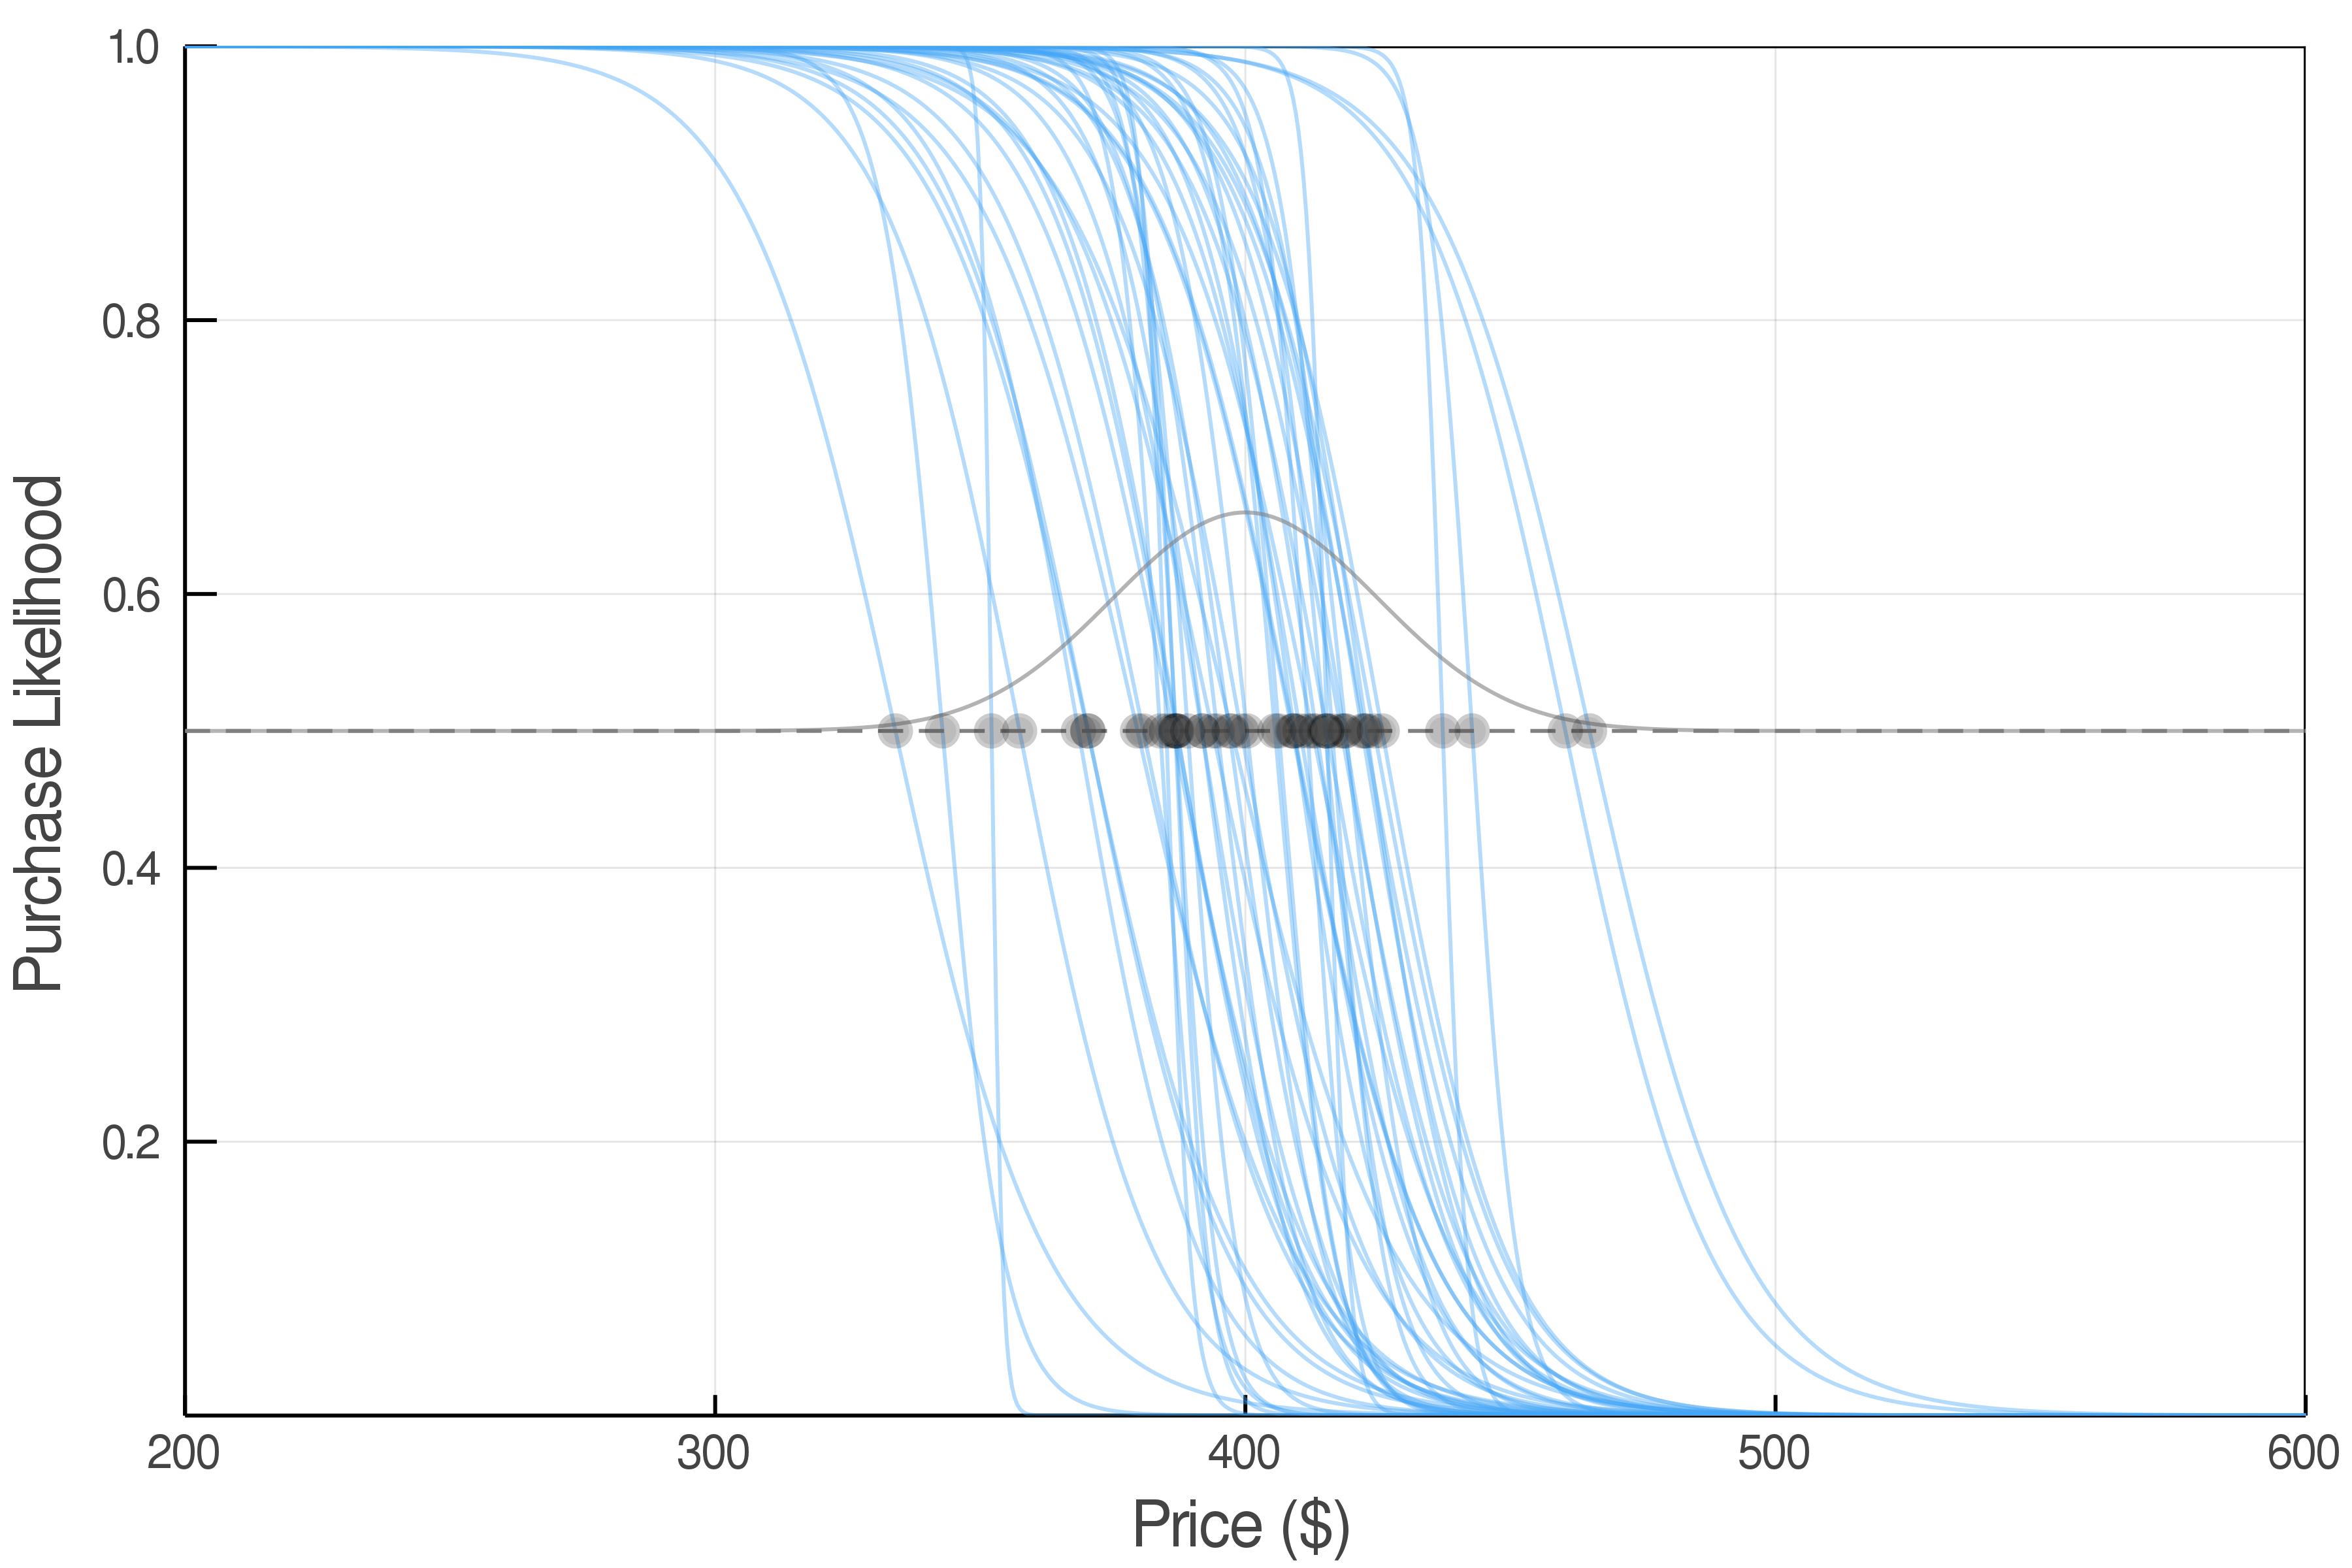
\includegraphics[width=0.9\linewidth]{plots/customer_price_schedule.png}
	\captionof{figure}{50 samples of customer purchasing schedules}
	\setlength{\belowcaptionskip}{-10pt}
    \label{fig:pricing-dynamics-example}
\end{Figure}
\vspace*{-0.1in}
\begin{Figure}
    \centering
    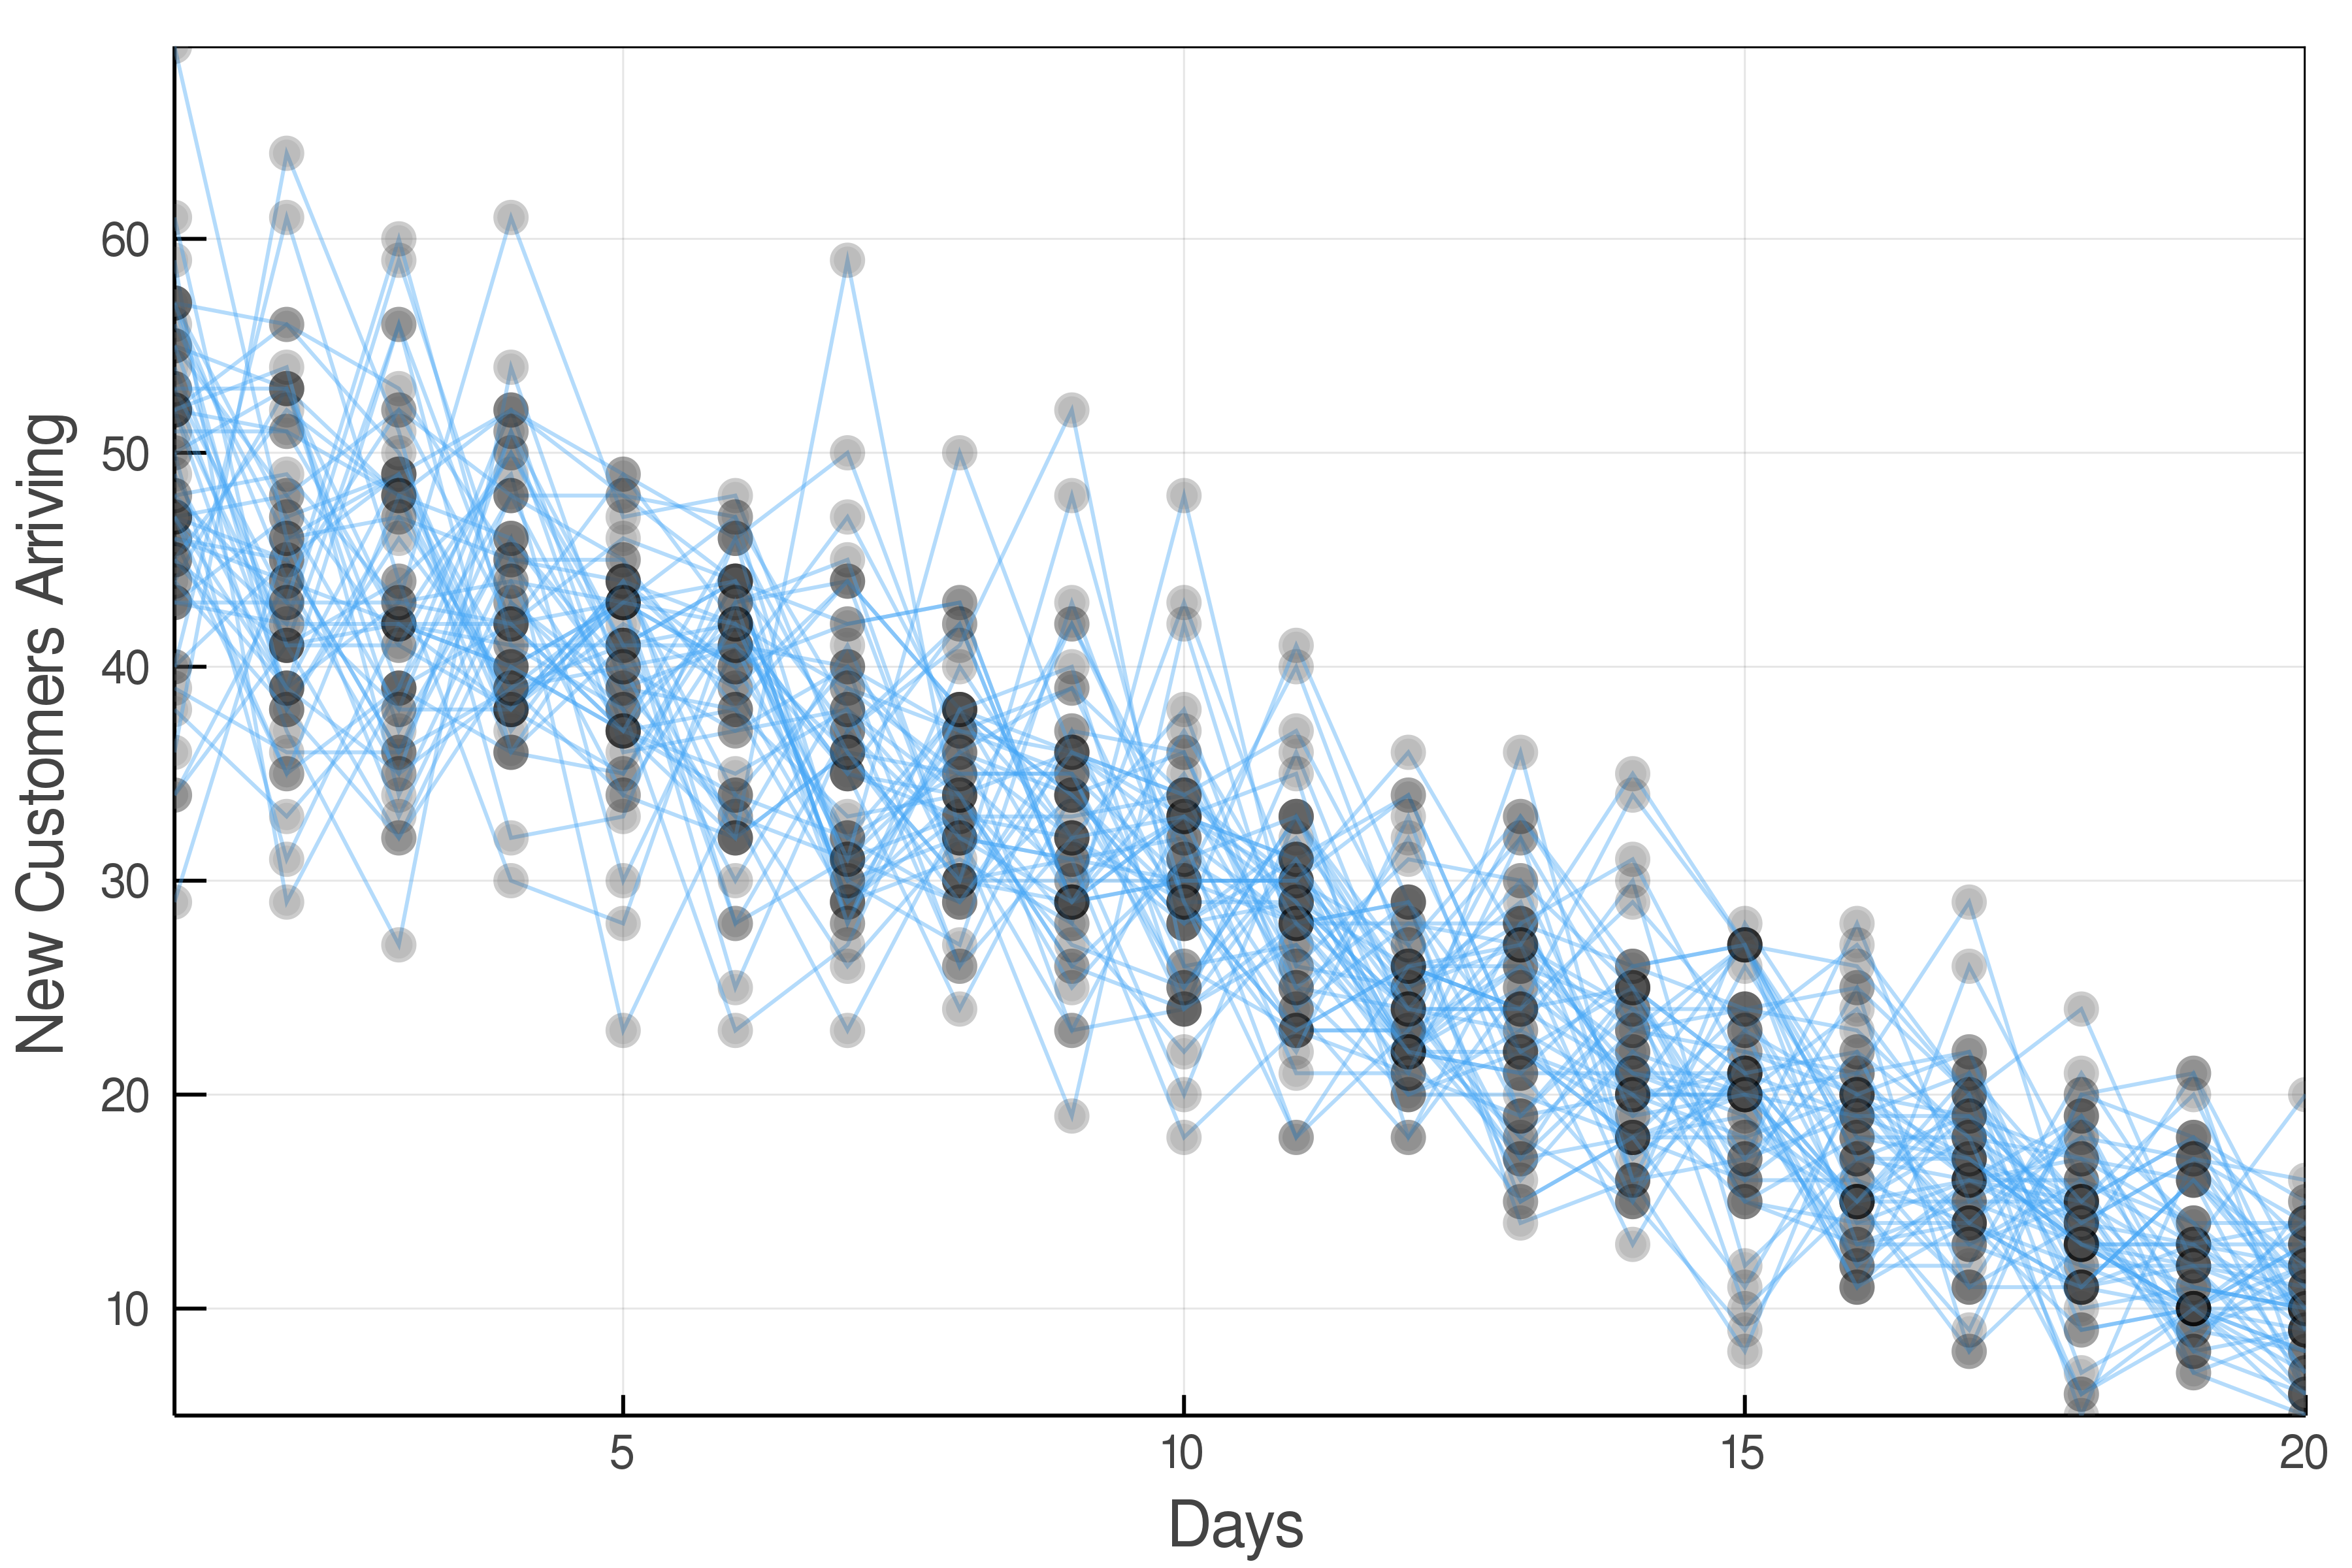
\includegraphics[width=0.9\linewidth]{plots/customer_arrival.png}
    \captionof{figure}{50 samples of the arrival of customers over a 20-day horizon}
    \setlength{\belowcaptionskip}{-10pt}
    \label{fig:arrival-dynamics-example}
\end{Figure}

We solve the overarching MDP using the Sarsa method, as shown in \hyperref[alg:solve-mdp]{Algorithm 2}. At each time step, we call the generative model for each fare class and add their contributions to get the next state $(v',h')$ and current reward $r$, then use the Sarsa update rule.

In line 9, we check to see if we have oversold our stock of tickets. If so, we correct it in line 10 by simulating selling the remaining tickets to customers on a first-come, first-served basis. E.g., if 15 customers wanted to buy from a remaining pool of 5 tickets, we would randomly pick 5 of the customers, independent of fare class, to obtain those tickets.

\begin{algorithm}[H]
\label{alg:solve-mdp}
	\caption{\textsc{SolveMDP}}
	\small\begin{algorithmic}[1]
        \State ${(v,h)} \leftarrow (V,H)$
    	\State ${r} \leftarrow 0$
    	\State Initialize $Q(s,a) = 0, \forall s \in S, a \in A$
    	\State Select $a$ using $\epsilon$-greedy with Gaussian randomness
    	\Repeat {}
        	\For {$f \in F$}
                \State $(v',u_f',h_f'),r_f \leftarrow$ 
                \textsc{GenerativeModel$_f ((v, 0, h), a)$}
            \EndFor
            \If {$\sum_f u_f' > v$}
     	        \State Randomly choose values for each $u_f'$ so that $\sum_f u_f' = v$
             \EndIf
             \State $(v', h') \leftarrow (v - \sum_f u_f', h - 1)$
    		\State $r \leftarrow \sum_f r_f$
    		\State Select $a'$ using $\epsilon$-greedy with Gaussian randomness
    		\State $Q(s,a) \leftarrow Q(s,a) + \eta(r_t + \gamma Q((v',h'),a') - Q(s,a))$
    		\State $s \leftarrow (v',h'), a \leftarrow a'$
     	\Until $h = 0$ or $v' = 0$
	\end{algorithmic}
\end{algorithm}

Finally, we can extract the optimal policy, $\pi^*$ using \hyperref[alg:extract-policy]{Algorithm 3}.

\begin{algorithm}[H]
\label{alg:extract-policy}
	\caption{\textsc{ExtractPolicy($Q$)}}
    	\small\begin{algorithmic}[1]
     	\For {$s \in S$}
     	    \State $\pi^*(s) \leftarrow {\arg\max}_a Q(s,a)$
     	\EndFor
        \State\Return {$\pi^*$}
	\end{algorithmic}
\end{algorithm}

\section*{Timeline to Completion}

First, we will continue to develop the generative model and then solve a single fare MDP. Following this, we will move to the multi-fare MDP formulation. We are using sarsa($\lambda$) to approximate the value function, though local or global approximation methods may be exploited later to improve generalization of the agent. We are on track to complete everything by December 6th.

% -------

% \textit{To consider}

% - Need to refine alg 1 to carry over the set C at every time step?
% I updated the text to say that C starts initially empty. I think we should be fine just leaving C as an overarching set - I've seen Mykel do this in the DMU book a few times where he just neglects some of the constants/sets from being passed in 

% - Does the Markov property still hold if we increase WTP over time?
% I don't think so - Markov property is time invariance (stationarity) of the problem dynamics. Even though WTP is stochastic, it is stationary. If we add some change later in the MDP, the WTP would be stochastic and non-stationary since the expected value & possibly variance would change with time.

% I put in my updates this morning and I think I'm pretty much satisfied with it! Feel free to make any small changes and if you're happy with it, could you submit it to Canvas this afternoon? Thanks! 

\end{multicols*}

\end{document}